\documentclass[12pt]{article}

\usepackage{graphicx}
\usepackage{fullpage}
\usepackage[utf8]{inputenc}
\usepackage[brazil]{babel}
\usepackage{amsmath}

\begin{document}

\begin{center}
\Large{DCC04 -- Red-Black Trees 1}
\end{center}

\vspace{1cm}

\noindent
Nome: \rule{8cm}{0.01in} \ Matr\'{i}cula: \rule{3cm}{0.01in}

\vspace{1cm}

%%%%%%%%%%%%%%%%%%%%%%%%%%%%%%%%%%%%%%%%%%%%%%%%%%%%%%%%%%%%%%%%%%%%%%%%%%%%%%%%

\begin{enumerate}

\item Assume that a binary search tree \texttt{Tree} contains the following
operations:

\begin{itemize}
\item \texttt{typedef struct Node *Tree}

\item \texttt{Reg* getReg(Tree t)}

\item \texttt{Tree getL(Tree t)}

\item \texttt{Tree getR(Tree t)}
\end{itemize}

Thus, any pointer \texttt{t}, having type \texttt{Tree}, is either \texttt{NULL},
or it is a tree-node.
In the latter case, we have the following properties:

\begin{itemize}
\item any element in the left subtree (\texttt{getL}) is less than the 
current element;
\item any element in the right subtree (\texttt{getR}) is greater than the 
current element.
\end{itemize}

Additionally, assume that a binary search tree is a {\em balanced} tree if
it contains this property:

\begin{itemize}
\item \texttt{abs(getL(t), getR(t)) $\leq$ 1}, where \texttt{abs} is the
absolute value of integers.
\end{itemize}

From these observations, implement a function \texttt{Tree balance(Tree t)},
which receives a tree \texttt{t}, and returns another tree that is balanced,
and contains all the elements in \texttt{t}.

\newpage

\item Transform each one of the trees below, so that it becomes a red-black
tree.
Remember, a red-black tree has these two core properties:

\begin{itemize}
\item Every path from the root till the leaf node contains the same number of
black nodes;
\item Every children of a red node is black.
\end{itemize}

Assume that \texttt{B} is the number of nodes in a subtree.
You should not assume that the PARENT node has any particular color: you must
prove that it has some color that lets you do the transformation. \\

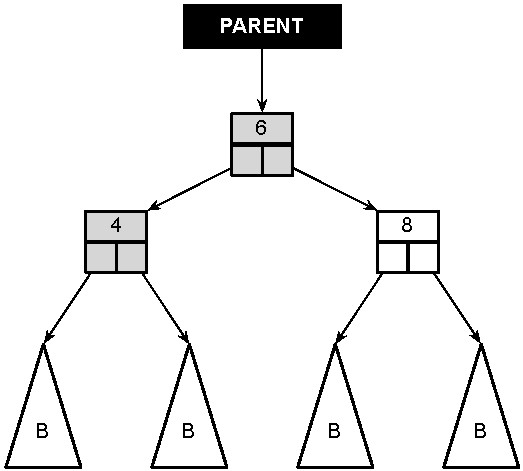
\includegraphics[scale=0.7]{images/RBT_1}

\vspace{2cm}

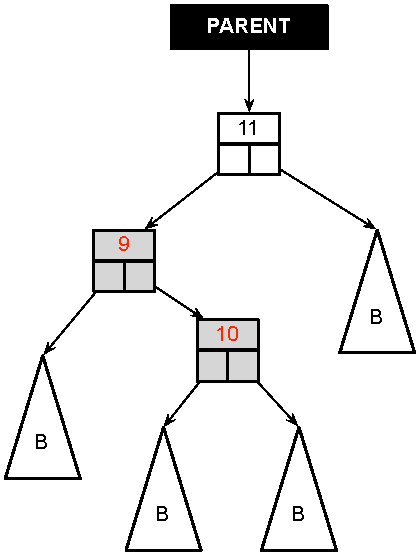
\includegraphics[scale=0.7]{images/RBT_2}

\end{enumerate}

\end{document}
